\begin{frame}{ATLAS run 1 H boson mass measurement}
\centering
$$m_H = 125.36 \pm 0.37 \text{(stat)} \pm 0.18 \text{(syst)}$$
\begin{minipage}{0.49\linewidth}
  \includegraphics[width=\linewidth]{1406_3827_8f.pdf}
\end{minipage}
\hfill
\begin{minipage}{0.49\linewidth}
  \begin{tikzpicture}
    \node[anchor=south west] { \includegraphics[width=\linewidth]{1406_3827_4t.pdf} };
%    \draw[step=1.0,black,thin] (0,0) grid (6,3);
    \draw[red, line width=0.5mm, rounded corners =2pt] ( 0.1, 1.05 ) rectangle ( 6.1, 1.35 ) ;
  \end{tikzpicture}
\end{minipage}
    {\bf Statistical uncertainties highly dominant.}\\
    \begin{center}   Run 2 will increase sensitivity to systematics.\end{center}
\end{frame}

%%========================================
\begin{frame}{$\mu_{\gamma\gamma}$ measurement}
%$\mu_{\gamma\gamma}$ is a main variable to measure. It is related to the cross section (production probability) :
$$\mu_{\gamma\gamma}=\frac{(\sigma\times BR)^{meas}}{(\sigma\times BR)^{SM}}=1.17 \pm 0.23 \text{(stat)}\ ^{+0.10}_{-0.08}\text{(syst)}\ ^{+0.12}_{-0.08} \text{(theory)}$$
  \begin{minipage}{0.49\linewidth}
    \includegraphics[width=\linewidth]{1408_7084_19f.pdf}
  \end{minipage}
  \hfill
  \begin{minipage}{0.49\linewidth}
    \begin{tikzpicture}
      \node[anchor=south west] { \includegraphics[width=\linewidth]{1408_7084_19t.pdf} };
%      \draw[step=1.0,black,thin] (0,0) grid (6,3);
      \draw[red, line width=1mm, rounded corners =2pt] ( 0, 0.75 ) rectangle (6, 1.6 ) ;
    \end{tikzpicture}
  \end{minipage}
If no improvements, \textcolor{blue}{\bf calibration uncertainty will be dominant in run 2}.
\end{frame}
%%=================================================================================
\begin{frame}{Reconstructed categories}
  \begin{minipage}{0.49\linewidth}
      \includegraphics[width=\linewidth]{ATL-COM-PHYS-2016-1784_flowchart-eps-converted-to.pdf}
  \end{minipage}
  \hfill
  \begin{minipage}{0.49\linewidth}
    Optimised sensitivity to :
    \begin{itemize}
    \item rare processes
    \item truth bins
    \end{itemize}
    \includegraphics[width=\linewidth]{ATLAS-CONF-2017-045_4t.pdf}
  \end{minipage}
\end{frame}

%%=================================================================================
\begin{frame}{Background parametrization}
  \begin{minipage}{0.45\linewidth}
    \includegraphics[width=\linewidth]{ATLAS-CONF-2017-045_3fa.pdf}
  \end{minipage}
  \hfill
  \begin{minipage}{0.45\linewidth}
    \begin{itemize}
    \item MC not reliable for background description
    \item Shape fitted on data
    \item Spurious signal (signal measured on background only sample) evaluated for selection of functional form.
    \end{itemize}
  \end{minipage}\\
  \includegraphics[width=0.9\linewidth]{ATL-COM-PHYS-2016-1784_52f.pdf}
\end{frame}

%%=================================================================================
\begin{frame}{Calibration uncertainties methodology}
  \begin{minipage}{0.49\linewidth}
    For a given systematic source :
    \begin{itemize}
    \item Create distributions of \\ $m_{\gamma\gamma}^{nom}$, $m_{\gamma\gamma}^{up}$, $m_{\gamma \gamma}^{down}$
    \item Fit main parameter of the systematic with DSCB :
      \begin{itemize}
      \item Fit  $m_{\gamma\gamma}\in[105,160]$GeV
      \item Fixing $n_{high}=5$ and $n_{low}=9$
      \item Fixing $\alpha_{high}=\hat{\alpha}_{high}^{nom}$, $\alpha_{low}^{nom}=\hat{\alpha}_{low}^{nom}$, $X=\hat{X}^{nom}$
%        \item Fixing secondary parameter to nominal fitted values.
      \end{itemize}
      \item Systematic variation : $\frac{X^{fluct}}{X^{nom}}-1$, $X\in \{\mu , \sigma\}$
      \end{itemize}
    \end{minipage}
    \hfill
    \begin{minipage}{0.49\linewidth}
      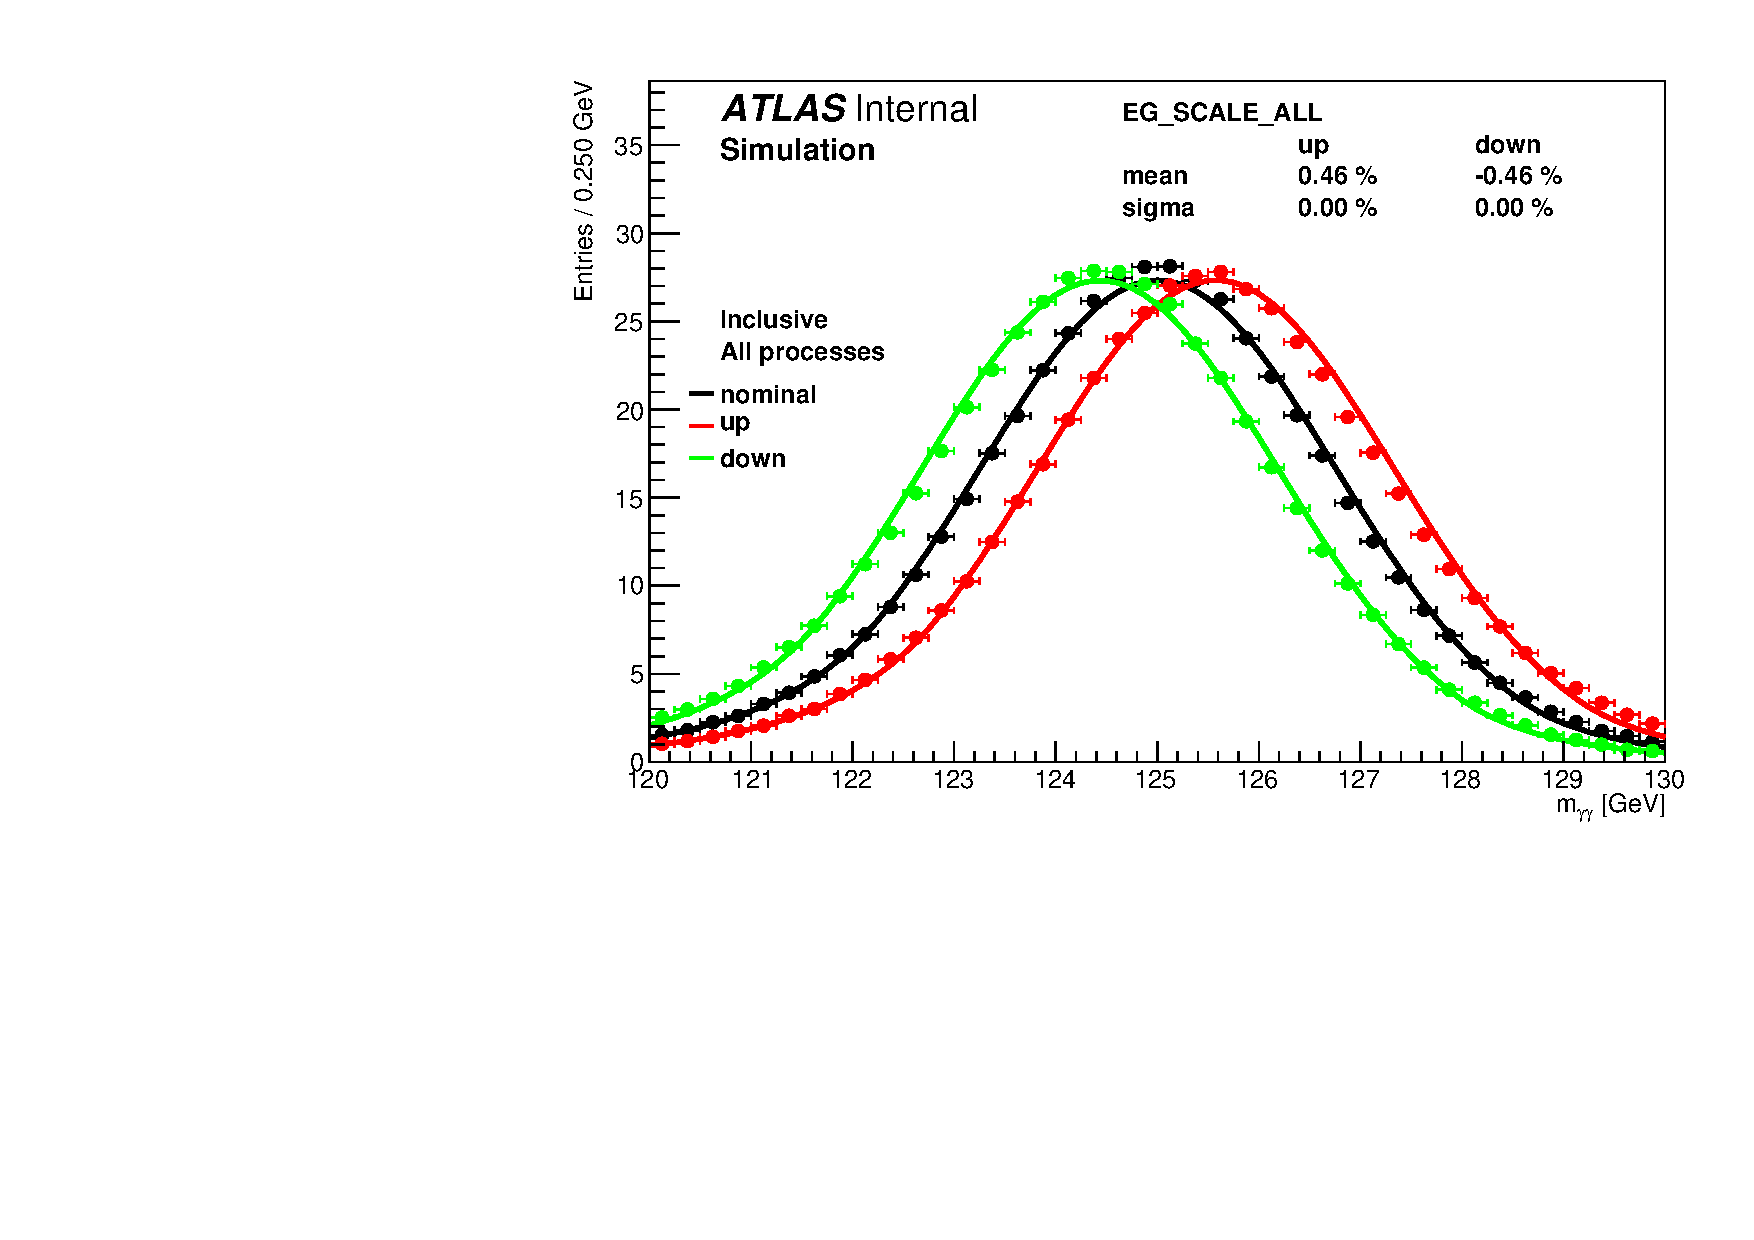
\includegraphics[width=\linewidth]{Figures/h013_EG_SCALE_ALL_0.pdf}
    \end{minipage}
    \vfill
    
    \begin{equation}
      \tiny
      CB(m_{\gamma \gamma}) = 
      \begin{cases}
        e^{-t^{2}/2} & \text{if } -\alpha_{low} \leq t \leq \alpha_{high} \\
        \frac{ e^{-{}^{1}_{2} \alpha_{low}^{2}} } { \left[ \frac{1}{R_{low}} \left(R_{low} - \alpha_{low} - t \right) \right]^{n_{low}} } & \text{if } t < -\alpha_{low} \\
        \frac{ e^{-{}^{1}_{2} \alpha_{high}^{2}} } { \left[ \frac{1}{R_{high}} \left(R_{high} - \alpha_{high} + t \right) \right]^{n_{high}} } & \text{if } t > \alpha_{high} \\
        t=(m_{\gamma\gamma}-\mu)/\sigma, R_{low}=\frac{\alpha_{low}}{n_{low}},  R_{high}=\frac{\alpha_{high}}{n_{high}} \\
      \end{cases}
    \end{equation}

%    More work required to improve fits quality.
\end{frame}
%%=================================================================================
\begin{frame}{Scale impact on width}
  \begin{minipage}{0.49\linewidth}\includegraphics[width=\linewidth]{/home/goudet/Documents/LAL/Zim/Hgam/PhotonSystematic/160826_SpreadGauss.pdf}\end{minipage}
  \hfill
  \begin{minipage}{0.49\linewidth}
    1M random numbers generated on a Gaussian$(\mu=125, \sigma=1)$.
    \begin{itemize}
    \item Initial numbers distribution.
    \item \textcolor{red}{Half events multiplied by $1.002$.}
    \item \textcolor{blue}{Remaining  events multiplied by $1.005$.}
    \item \textcolor{magenta}{Combined distribution of \textcolor{red}{red} and \textcolor{blue}{blue}.}
    \end{itemize}
  \end{minipage}
  \vfill
  Mean (m) and RMS (s) of a fitted gaussians are given in the legend.
  Interpretationof the curve in the next slides.
\end{frame}

%%=================================================================================
\begin{frame}{$\mu /\sigma$ scale correlation}
  \begin{minipage}{0.49\linewidth}\includegraphics[width=\linewidth]{/home/goudet/Documents/LAL/Zim/Hgam/PhotonSystematic/160826_SpreadGauss.pdf}\end{minipage}
  \hfill
  \begin{minipage}{0.49\linewidth}
    Lets assume a gaussian distributed energy distribution.
    Applying energy scale correction gives : $$E\rightarrow E(1+a)$$

  \end{minipage}
      Hence the distribution will be changed to  :
      \begin{equation}
      exp( -\frac{(E-\mu)^2}{2\sigma^2}\
      \rightarrow\
      exp( -\frac{(\frac{E}{1+a}-\mu)^2}{2\sigma^2})
      =
      exp( -\frac{(E-\mu(1+a))^2}{2\sigma^2(1+a)^2})
    \end{equation}
      The new distribution is a \textcolor{red}{shifted gaussian with scaled RMS}.\\
      Given the medium shift of EG\_SCALE\_ALL, we expect \textcolor{red}{$^{+0.4}_{-0.4}\%$} change in resolution.
\end{frame}


%%=================================================================================
\begin{frame}{Inhomegenous scale}
  \begin{minipage}{0.49\linewidth}\includegraphics[width=\linewidth]{/home/goudet/Documents/LAL/Zim/Hgam/PhotonSystematic/160826_SpreadGauss.pdf}\end{minipage}
  \hfill
  \begin{minipage}{0.49\linewidth}
    The RMS of two points separated by $d$ is $d/4$.\\
    If $d$ is the difference between two scale factors, $$d\sim 3.10^{-3} \cdot E_\gamma=0.18$$
   $$\frac{\text{RMS}}{\text{Resolution}} = \frac{d/4}{1.5\text{GeV}} = 3\%$$
  \end{minipage}
\vfill
  The inhomogeneity of the scale factors uncertainties \textcolor{red}{changes the width of the distribution at the percent level}.
  This effect will always increase the width.  
  \vfill
  Black and pink distribution show an illustration of this effect.
\end{frame}

%==============================================================================
\begin{frame}{Scale factors interpretation}
  \begin{minipage}{0.49\linewidth}
    Assume the up fluctuation (red) as data and nominal distribution (black) as MC in the template method.
    One has
    $$m_H^{up}=m_H^{nom}(1+\alpha)$$
    Hence
    $$\delta_{m_H}=\alpha$$
    \end{minipage}
  \begin{minipage}{0.49\linewidth}
    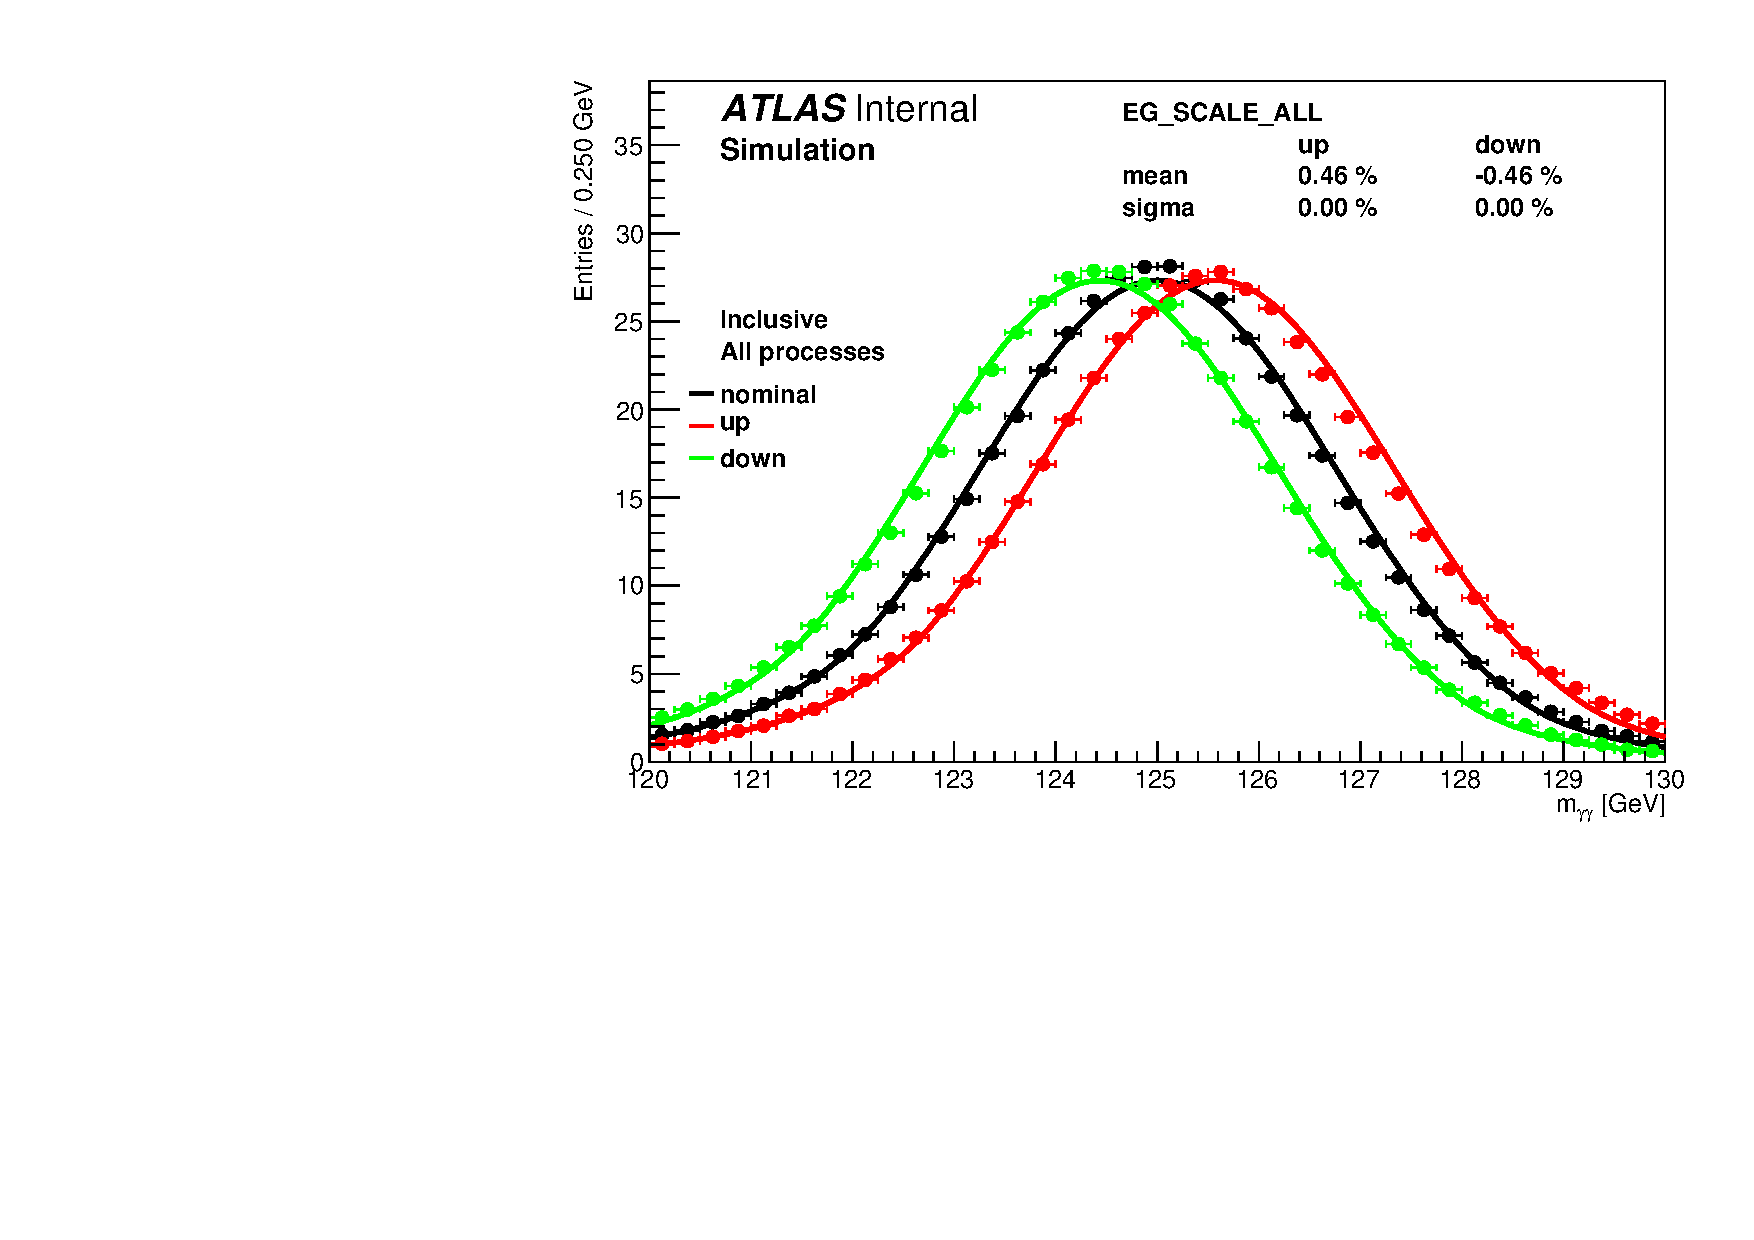
\includegraphics[width=\linewidth]{Figures/h013_EG_SCALE_ALL_0.pdf}
  \end{minipage}
  Furthermore :
  $$\sigma_H^{up}=\sigma_H^{nom} \oplus cE$$
  Hence
  $$\delta_{\sigma_H} = \sqrt{1+\frac{c^2E^2}{\sigma_H^2}}-1$$
  One has to be carefull with resolution uncertainty as the template method is weak to measure small differences.
\end{frame}

%%=================================================================================
\begin{frame}{Method comparison}
  4 different fitting methods are compared : fitting in 3 different ranges and template method cross-check within $[122, 128]$GeV.
  Methods compared on h013 simplified model (2NP).
  
  \begin{minipage}{0.42\linewidth}
   % $$m_{\gamma\gamma}\in [105,160]$$
    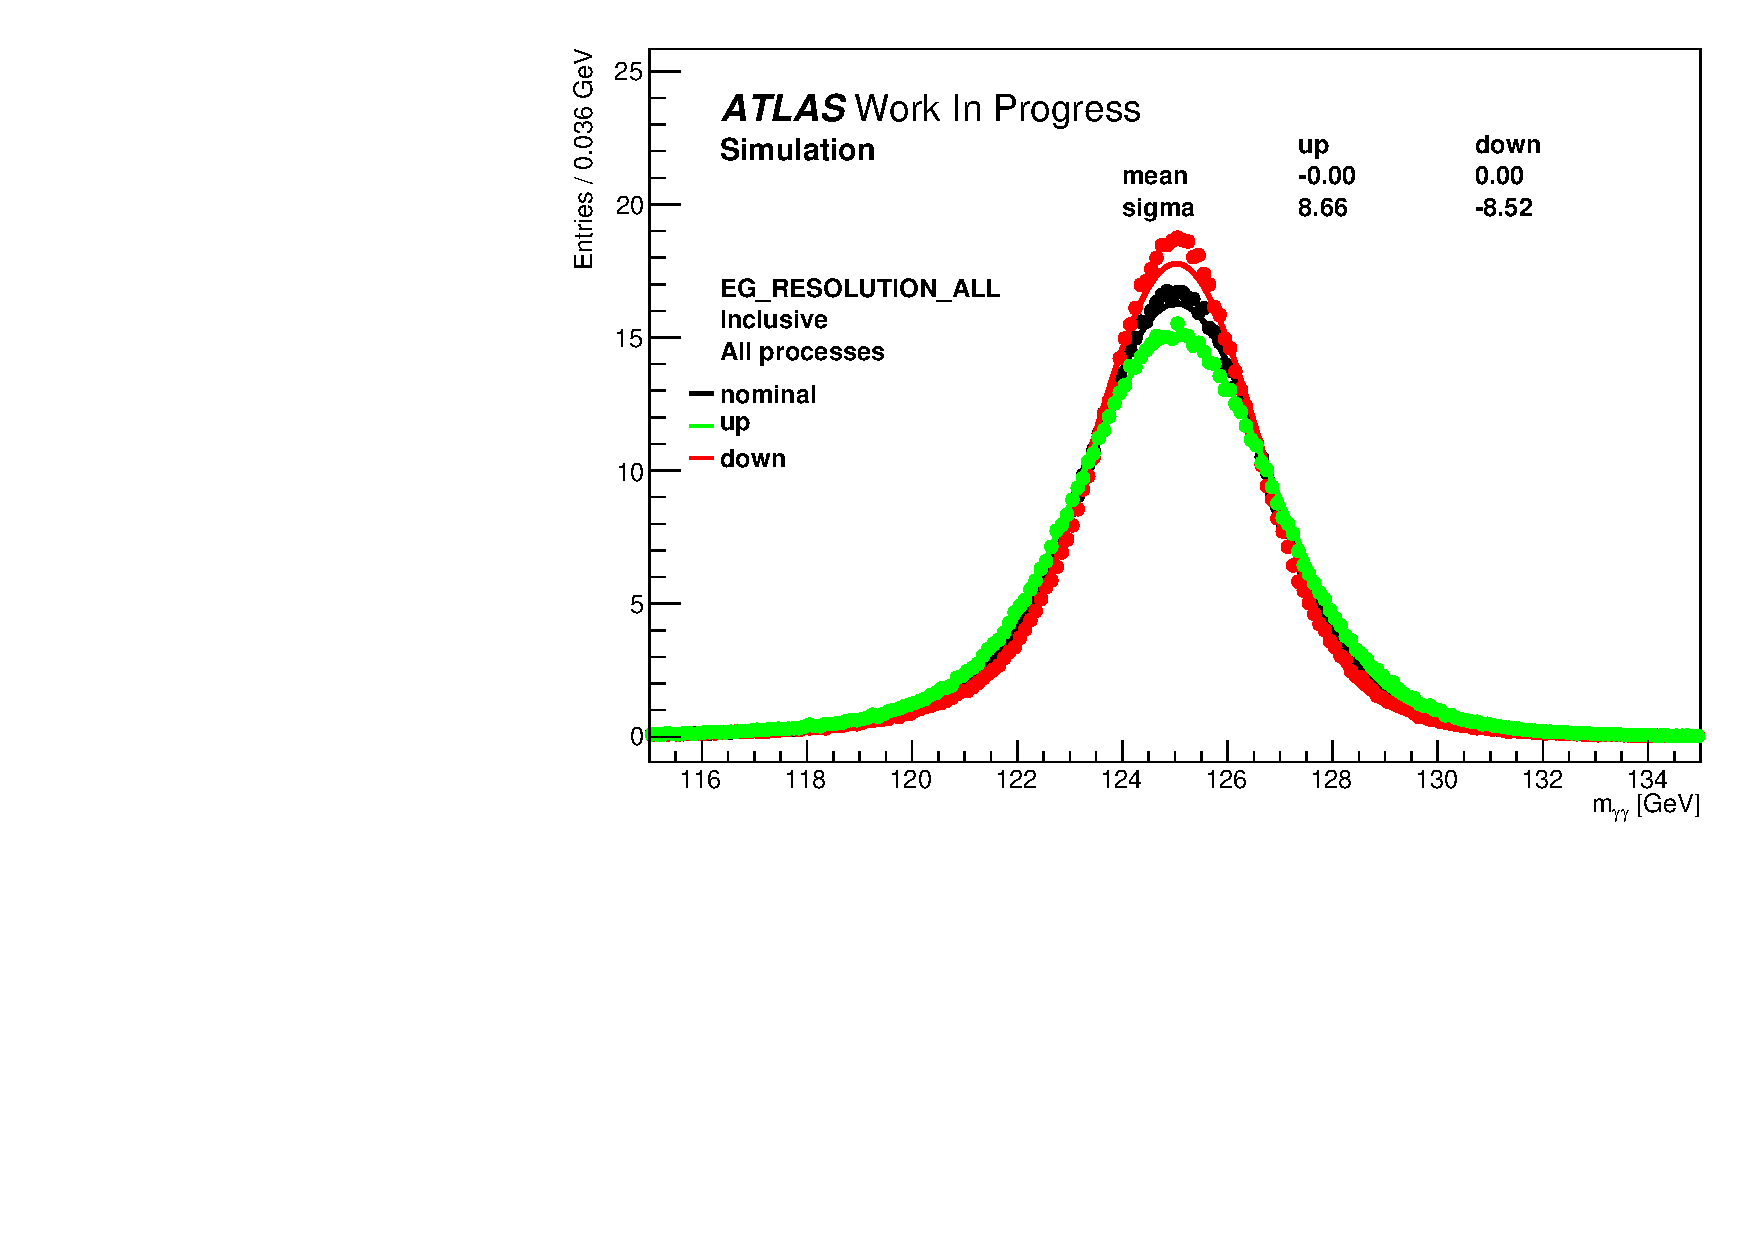
\includegraphics[width=\linewidth]{Figures/h013_EG_RESOLUTION_ALL_0_105160.pdf}
  \end{minipage}
  \hfill
  \begin{minipage}{0.14\linewidth}
    $\leftarrow [105,160]$
    $\rightarrow [115,135]$
    \end{minipage}
  \hfill
  \begin{minipage}{0.42\linewidth}
    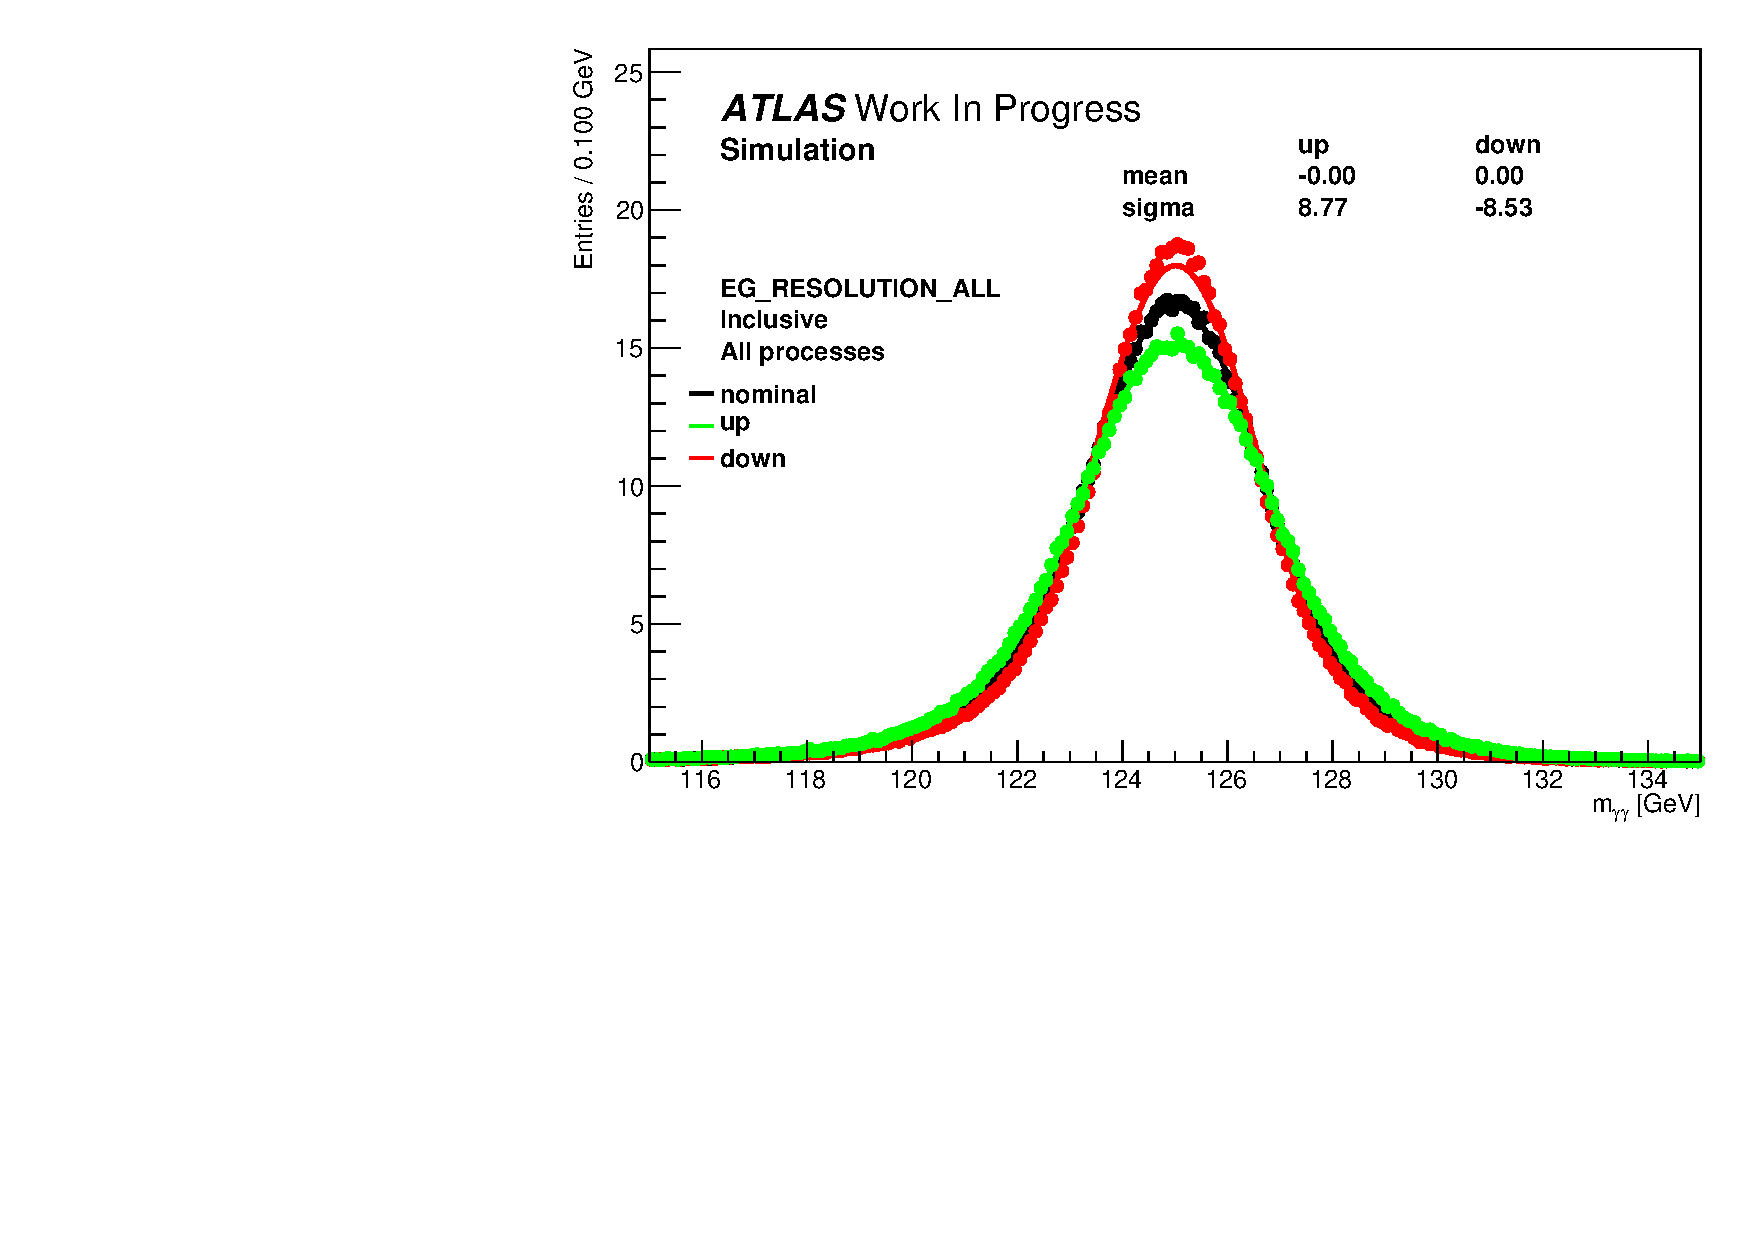
\includegraphics[width=\linewidth]{Figures/h013_EG_RESOLUTION_ALL_0_115135.pdf}
  \end{minipage}
  \begin{minipage}{0.42\linewidth}
    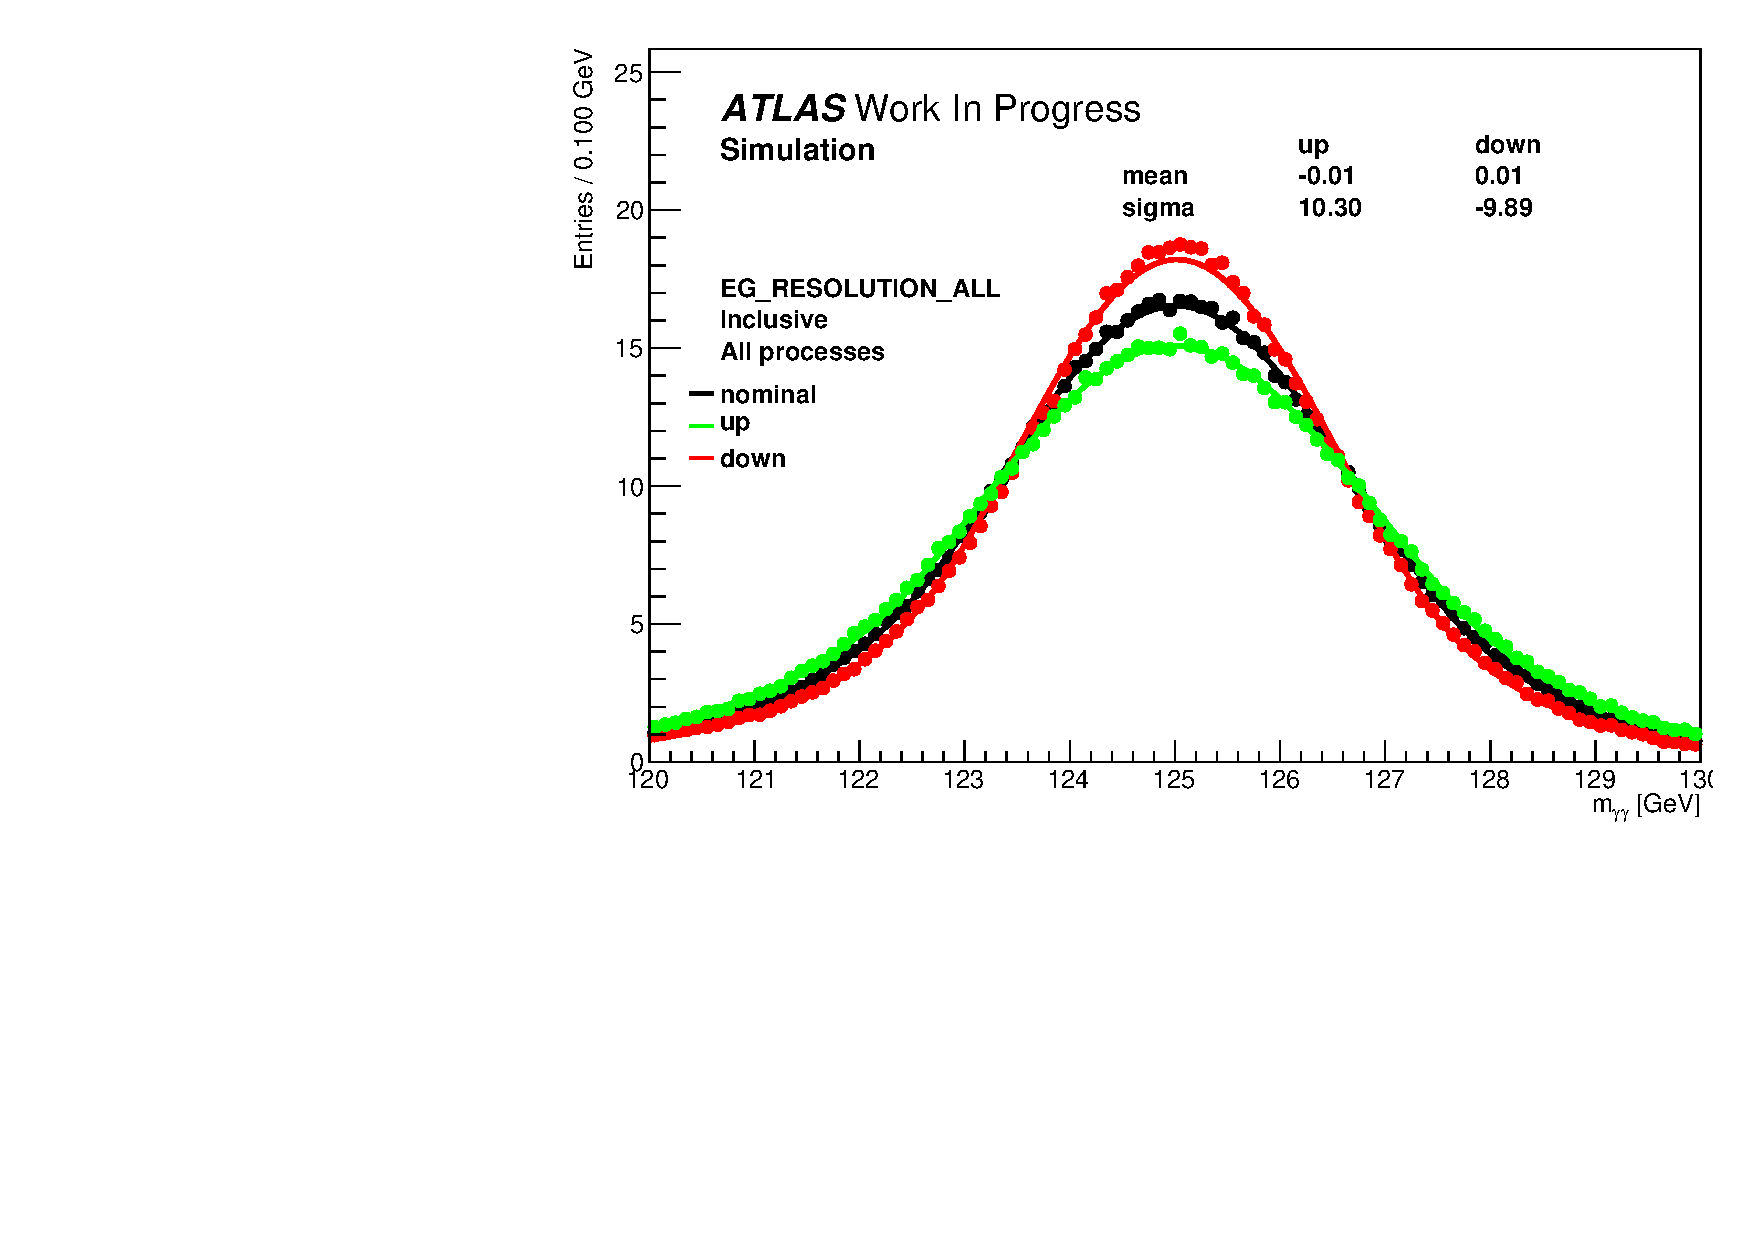
\includegraphics[width=\linewidth]{Figures/h013_EG_RESOLUTION_ALL_0_120130.pdf}
  \end{minipage}
  \hfill
  \begin{minipage}{0.14\linewidth}
    $\leftarrow [120,130]$
    $\rightarrow [122,128]$
  \end{minipage}
    \hfill
  \begin{minipage}{0.42\linewidth}
    \centering
        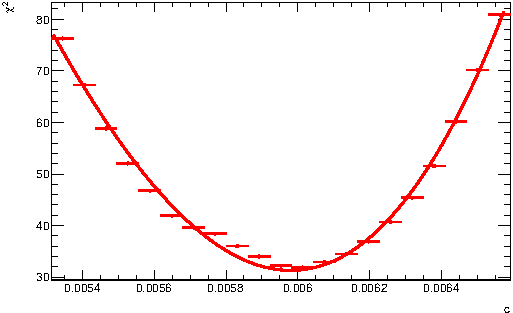
\includegraphics[width=0.5\linewidth]{Figures/h013_EG_RESOLUTION_ALL__1up_0_scale.pdf}\\
        $c=(0.598\pm 0.009)\%$\\$\rightarrow \delta_{\sigma_H}=(8.82\pm0.25)\%$
  \end{minipage}
\end{frame}
%========================================================================
\begin{frame}{Uncertainty correlation formula}
\centering
\begin{equation}
  \frac{\sigma(M)}{M} = \frac{1}{N_\gamma}\sqrt{\sum_{ij}N_iN_jV_{ij}}.
  \label{eq:HGam_covariance}
\end{equation}

\includegraphics[width=0.6\linewidth]{ATL-COM-PHYS-2016-1784_systematics_shape_Unal_mh_syst_corrFULL.pdf}\\

 \resizebox{0.6\linewidth}{!}{
\begin{tabular}{l|ll}
Total Scale Uncertainty (\%) & 1NP & FULL \\
\hline
Measurement with $H\rightarrow\gamma\gamma$ MC & 0.46 & 0.27\\
Formula & 0.47 & 0.26\\
\end{tabular}
}

\end{frame}

%==========================================================
\begin{frame}{Likelihood Method}
A function ({\bf likelihood}) is built to {\bf evaluate the best set of parameters ($\vec{\mu}$,$\vec{\theta}$)} of a model to agree the best with a dataset in a category.

$$\mathcal{L}=\underbrace{\frac{(n_{s}(\vec{\mu},\vec{\theta})+b)^{n_{obs}}}{n_{obs}!} e^{-(n_{s}(\vec{\mu},\vec{\theta})+b)}}_{\textcolor{red}{\text{(1)}}}  \overbrace{\prod_j^{n_{obs}}\psi(\vec{x_j};\vec{\mu},\vec{\theta})}^{\textcolor{violet}{\text{(2)}}} \underbrace{e^{-\frac{\theta^2}{2}}}_{\textcolor{blue}{\text{(3)}}}$$
\vfill
\begin{minipage}{0.49\linewidth}
\textcolor{red}{(1) {\bf Poissonian law} to evaluate the probability to observe $n_{obs}$($\equiv$ signal $+$ background) events when $(n_s+b)$ are expected.}\newline
\textcolor{violet}{(2) {\bf Probability density function} of the observables $\vec{x}$ (diphoton invariant mass for example) for the $j^{th}$ event.}\newline
\textcolor{blue}{(3) Constraint on the nuisance parameter $\theta$. See next slide.}\newline
\end{minipage}
\begin{minipage}{0.49\linewidth}
\includegraphics[width=\linewidth]{Cgam_009.png}
\end{minipage}
\end{frame}
%%==========================================================

\begin{frame}{Nuisance parameters}
There are some {\bf external measurements}  that contribute to the likelihood and have some {\bf uncertainties}. 
A {\bf free nuisance parameter} is added for each of these measurements.
In order  to take into account these external measurements, a {\bf constraint is put on these nuisance parameters}. 
\vfill
For example, the luminosity is re-defined as  $L(1+\delta_L \theta_L)$, with $\theta_L$ the nuisance parameter and $\delta_L$ the uncertainty on the luminosity (assumed to be Gaussian).
In this case, a Gaussian constraint is chosen.

The contribution from luminosity will hence be :
$$L(1+\delta_L \theta_L)e^{-\theta_L^2/2}$$
\vfill
\textcolor{blue}{\bf Error Estimation}\newline
A test statistic is defined as : $t_\mu=-2ln\frac{\mathcal{L}(\mu,\hat{\hat{\theta}})}{\mathcal{L}(\hat{\mu},\hat{\theta})}$, with $\hat{\theta}$ and $\hat{\mu}$ the best (fitted) parameters, and $\hat{\hat{\theta}}$ the fitted nuisance parameters for a fixed $\mu$.\newline
Uncertainty are given by : \textcolor{red}{$\mathbf{t_{\hat{\mu}\pm 1\sigma}=1}$} and \textcolor{red}{$\mathbf{t_{\hat{\mu}\pm 2\sigma}=4}$} in 1D Gaussian limit.
\end{frame}
%%====================================================================
\begin{frame}{ATLAS $H\rightarrow 4l$ couplings measurement}

  \begin{center} \href{https://cds.cern.ch/record/2273849}{\bf ATLAS-CONF-2017-043} \end{center}
  
  \begin{minipage}{0.49\linewidth}
    \includegraphics[width=\linewidth]{ATLAS-CONF-2017-043_7fb.pdf}
  \end{minipage}
  \hfill
  \begin{minipage}{0.49\linewidth}
    \includegraphics[width=\linewidth]{ATLAS-CONF-2017-043_7fb.pdf}
    \end{minipage}
\end{frame}

%%====================================================================
\begin{frame}{CMS $H\rightarrow 4l$ couplings measurement}

  \begin{center} \href{http://cds.cern.ch/record/2272260}{\bf CMS-HIG-16-041} \end{center}
  
  \begin{minipage}{0.49\linewidth}
    \includegraphics[width=\linewidth]{CMS-HIG-16-041_8fa.pdf}
  \end{minipage}
  \hfill
  \begin{minipage}{0.49\linewidth}
    \includegraphics[width=\linewidth]{CMS-HIG-16-041_8fb.pdf}
    \end{minipage}
\end{frame}

%%====================================================================
\begin{frame}{CMS $H\rightarrow \gamma\gamma$ couplings measurement}

  \begin{center} \href{https://cds.cern.ch/record/2264515}{\bf CMS-PAS-HIG-16-040} \end{center}
  
  \begin{minipage}{0.49\linewidth}
    \includegraphics[width=\linewidth]{CMS-PAS-HIG-16-040_16f.pdf}
  \end{minipage}
  \hfill
  \begin{minipage}{0.49\linewidth}
    \includegraphics[width=\linewidth]{CMS-PAS-HIG-16-040_17f.pdf}
    \end{minipage}
\end{frame}

%%====================================================================
\begin{frame}{Run 2 H boson mass measurement}
  \begin{minipage}{0.58\linewidth}
  \centering
    ATLAS\\
    \includegraphics[width=\linewidth]{ATLAS-CONF-2017-046_8t.pdf}
    \vfill
    CMS\\
    $H\rightarrow 4l : 125.26 \pm 0.20 \text{(stat.)} \pm 0.08 \text{(syst)}$ \\
    $H\rightarrow \gamma\gamma : 125.4 \pm 0.15 \text{(stat.)} \pm 0.3 \text{(syst)}$ \\
  \end{minipage}
  \hfill
  \begin{minipage}{0.41\linewidth}
    \includegraphics[width=\linewidth]{CERN-EP-2016-100_18f.pdf}
  \end{minipage}
\end{frame}
